\documentclass{article}
% --- watermark (auto-inserted) ---
\usepackage{xcolor}
\usepackage{xfp}% \fpeval; in the kernel since 2022, harmless on older LaTeX
\usepackage{draftwatermark}
\newlength{\watermarkTextWidth}
\AddToHook{begindocument/end}{%
  \SetWatermarkText{\normalfont Generated by The Agentic Scientist}%
  \SetWatermarkFontSize{10pt}%
  \SetWatermarkLightness{0.85}%
  \settowidth{\watermarkTextWidth}{\normalfont\fontsize{10pt}{12pt}\selectfont Generated by The Agentic Scientist}%
  \edef\watermarkScale{\fpeval{0.8 * sqrt(\paperwidth**2 + \paperheight**2) / \watermarkTextWidth}}%
  \edef\watermarkAngle{\fpeval{atand(\paperheight/\paperwidth)}}%
  \SetWatermarkScale{\watermarkScale}%
  \SetWatermarkAngle{\watermarkAngle}%
}
% --- end watermark ---

\usepackage{paper,times}
\usepackage{amsmath,amssymb,booktabs,graphicx,subcaption,url}
\usepackage[hidelinks]{hyperref}
\title{Local Residual Scaling for Compositional Conformal Prediction: Benefits and Limits}
\author{Anonymous authors}
\newcommand{\ilr}{\operatorname{ilr}}
\newcommand{\softmax}{\operatorname{softmax}}
\newcommand{\E}{\mathbb{E}}
\newcommand{\R}{\mathbb{R}}
\begin{document}
\maketitle

\begin{abstract}
Predictive regions for compositions must describe uncertainty jointly over a vector constrained to the simplex. We study when training-only local residual scaling improves split-conformal prediction in isometric log-ratio coordinates. The frozen procedure selects among a quadratic log-residual ridge model, a constant scale, and blends with additive quantile stumps, without using calibration outcomes. Six independent seeds evaluate continuous logistic-normal responses in dimensions three and ten under homoscedasticity, boundary-concentrated heteroscedasticity, and a test-covariate shift. Mean evaluation utility is 0.87723, compared with 0.82960 for global log-ratio calibration; the paired seed-bootstrap interval for the difference is [0.04390, 0.05062]. Benefits concentrate in heteroscedastic conditions, while homoscedastic conditions show no consistent advantage. Improved empirical coverage under the tested shift does not establish validity under distribution shift, and the shifted three-part condition uses more reference mass than global calibration. These results support condition-dependent scale adaptation, not component-specific superiority or uniformly smaller regions.
% @evidence[[paper_data.json#/final_evaluation]]
% @evidence[[paper_data.json#/final_evaluation/evaluation_evidence/episodes/0/solution/paired_seed_intervals]]
\end{abstract}

\section{Introduction}
Compositions represent proportions of a whole: each coordinate is nonnegative and the coordinates sum to one. A predictive region for a composition should therefore contain a complete response vector, not merely a collection of independently plausible coordinates. The simplex constraint also changes the interpretation of distance. Absolute differences and relative differences need not identify the same departures, particularly when some components are small. Compositional analysis provides log-ratio representations for this purpose \citep{Aitchison1982,Egozcue2003}. Here the prediction target is a continuous composition observed with covariates. It is neither a discrete class label nor an unobserved probability vector inferred from multinomial counts.

Split-conformal prediction offers a useful separation of responsibilities: a fitted model proposes a score, and an independent calibration sample sets a threshold with a marginal coverage guarantee under exchangeability \citep{Vovk2005,Papadopoulos2002,Lei2018,AngelopoulosBates2021}. That guarantee does not select an efficient geometry, eliminate variation in coverage between groups, or survive arbitrary distribution shift. A globally calibrated residual norm can allocate too much radius to low-noise covariates and too little to high-noise covariates. A positive covariate-dependent scale is a simple way to adapt the radius without changing the calibration principle. Whether the resulting regions are preferable still depends on what is measured and where they are deployed.

Our research question is therefore specific: \emph{when does a training-only scale-selection procedure improve the coverage--reference-mass tradeoff of joint compositional prediction regions, and what do homoscedastic and shifted controls reveal about its limits?} We evaluate one fixed procedure and matched baselines, rather than proposing a new conformal guarantee or surveying all uncertainty methods. The response representation, fitted center, calibration data, test examples, and reference probes are shared across comparisons wherever their definitions permit.

The contributions are threefold. First, we specify a reproducible evaluation that separates marginal coverage, fixed-group coverage, and reference-measure efficiency for joint responses. Second, matched repeated evaluations show a useful distinction between homoscedastic and heteroscedastic conditions: local scaling improves the measured tradeoff in the latter but offers no consistent benefit in the former. Third, a shift stress test exposes the difference between empirical coverage repair and a distribution-free validity claim. These contributions concern the complete procedure, not isolated components.

\begin{figure}[t]
\centering

\includegraphics[width=\textwidth]{figures/conceptual_overview.png}
\caption{Joint compositional prediction with separated information roles. Independent center and scale training precede calibration of normalized log-ratio residuals. Matched evaluation separates coverage, fixed-group diagnostics, and reference mass. Exchangeability supports marginal calibration, not an unconditional claim about the shifted setting.}
\label{fig:overview}
\end{figure}

\section{Related Work}
\paragraph{Conformal prediction and adaptation.}
The conformal framework and its inductive formulation establish the calibration perspective used here \citep{Vovk2005,Papadopoulos2002}. Distribution-free regression and prediction-band constructions clarify the distinction between coverage guarantees and statistical efficiency \citep{Lei2018,LeiWasserman2014}. Locally adaptive scores and conformalized quantile regression motivate adapting uncertainty to heteroscedasticity \citep{AngelopoulosBates2021,Romano2019}. Our procedure predicts a scalar residual-norm scale; it does not fit lower and upper response quantiles as in conformalized quantile regression. Nor does it implement localized calibration weights \citep{Guan2023} or leave-one-out refitting such as jackknife+ \citep{Barber2021}. These methods provide context, not additional evaluated baselines.

\paragraph{Composition and conditional scale estimation.}
Logistic-normal distributions provide a continuous model on the interior simplex \citep{AitchisonShen1980}; log-ratio analysis avoids treating constrained coordinates as unconstrained measurements \citep{Aitchison1982}. The isometric transform supplies Euclidean coordinates for relative geometry \citep{Egozcue2003}. Within that representation, our scale family combines ridge regularization \citep{HoerlKennard1970} with quantile-loss fitting \citep{KoenkerBassett1978,KoenkerHallock2001} and shallow additive updates motivated by boosting \citep{Friedman2001,Friedman2002}. Quantile regression forests are a different conditional-quantile approach \citep{Meinshausen2006}; we do not evaluate forests. Cross-validation and conservative model selection are standard tools rather than novel contributions \citep{Stone1974,Hastie2009}.

\paragraph{What reliability can mean.}
Conditional-validity distinctions matter even when marginal calibration is theoretically justified \citep{Vovk2012,BarberLimits2021}. We therefore report fixed-group discrepancies without claiming distribution-free conditional coverage. Weighted conformal methods under covariate shift require additional structure \citep{Tibshirani2019}; robustness beyond exchangeability is a separate methodological problem \citep{BarberBeyond2023}. We implement neither correction. Finally, Wilson intervals and bootstrap summaries quantify different sources of empirical uncertainty \citep{Wilson1927,Efron1979}: the former describe individual coverage proportions, whereas our main comparative interval resamples independent seeds. No literature comparison is used as a substitute for a measured experimental comparison.

\section{Method}
\subsection{Problem Setup and Joint Regions}
Let $X\in\R^p$ and let $Y$ lie in the interior simplex
$\Delta^{D-1}_{\circ}=\{y\in(0,1)^D:\sum_j y_j=1\}$.
Choose $V\in\R^{D\times(D-1)}$ satisfying $V^\top V=I$ and $V^\top\mathbf{1}=0$. Define
\begin{equation}
 Z=\ilr(Y)=V^\top\log Y,\qquad
 \ilr^{-1}(z)=\softmax(Vz).
\end{equation}
The evaluator uses an orthonormal contrast basis and verifies its orthogonality, zero sums, and transform inversion. A fitted center $\widehat m(x)$ predicts $Z$, and a separately fitted positive scale $\widehat s(x)$ predicts the magnitude of its residual. All evaluated methods use the same center. Consequently, the main local-versus-global comparison changes residual scaling, not point prediction.
% @evidence[[source_evidence/evaluate_final.py#L566-L601]]

For a calibration set of size $n_c$, write
\begin{equation}
 R_i=\frac{\|Z_i-\widehat m(X_i)\|_2}{\widehat s(X_i)},\quad
 k_\alpha=\left\lceil(n_c+1)(1-\alpha)\right\rceil,\quad
 q_\alpha=R_{(k_\alpha)}.
 \label{eq:calibration}
\end{equation}
When $k_\alpha>n_c$, the threshold is $+\infty$, not the largest observed score. The prediction region is
\begin{equation}
 C_\alpha(x)=\left\{y\in\Delta^{D-1}_{\circ}:\|\ilr(y)-\widehat m(x)\|_2
              \le q_\alpha\widehat s(x)\right\}.
 \label{eq:region}
\end{equation}
Coverage is the event that the entire response belongs to this set. It is not average coordinate coverage. Set construction, finite-sample quantiles, and membership are owned by the evaluator; the scale learner receives only training covariates and training residual norms.
% @evidence[[source_evidence/evaluate_final.py#L581-L586]]
% @evidence[[source_evidence/scale_learner.py#L1-L20]]

\subsection{Design Rationale and Scale Selection}
The scale hypothesis is that an approximately multiplicative residual law,
$\|Z-\widehat m(X)\|_2\approx s_*(X)U$, can be made more homogeneous by dividing by an estimate of $s_*$. This is a modeling rationale, not a verified factorization. If residual size is already constant across covariates, adaptation should add little and can introduce estimation noise. If the same residual mechanism holds after a covariate shift, normalization may also help empirically, but approximation alone is not an exchangeability guarantee.

The inspected learner fits $T_i=\log\max(r_i,10^{-12})$, where $r_i$ is a training residual norm. Its reference model regresses log residuals on an intercept, standardized covariates, and their coordinatewise squares, with ridge penalty 2 on non-intercept coefficients. A second model estimates the conditional 0.9 quantile of log norms using additive decision stumps. It starts from the empirical target quantile and adds at most 80 updates with learning rate 0.1. For each covariate, 15 empirical split quantiles between 0.05 and 0.95 are considered. Each leaf must contain at least $\max(20,\lceil0.03n\rceil)$ fitting observations. The selected split minimizes mean pinball loss after its shrunken update; fitting stops when no numerical loss improvement remains.
% @evidence[[source_evidence/scale_learner.py#L84-L155]]

Candidate log scales are the ridge prediction, a constant, and ridge--stump blends with stump weights 0.25, 0.5, 0.75, and 1. An additive offset aligns each candidate using its fitting-set 0.9 quantile of log residual minus predicted log scale. Selection uses three disjoint folds from a fixed permutation. Each fold refits both component models and all offsets using only its fitting partition. Held-out mean pinball loss is computed as
\begin{equation}
 \rho_\tau(u)=\max\{\tau u,(\tau-1)u\},\qquad \tau=0.9.
\end{equation}
The candidate order is ridge, constant, then increasing stump weight. The learner takes the earliest candidate whose mean fold loss is within one estimated standard error of the minimum-loss candidate. It finally refits on all scale-training data. This ordering favors the existing ridge model, not the constant, when both satisfy the rule. The complete candidate list is fixed before held-out evaluation; final outcomes do not tune its hyperparameters.
% @evidence[[source_evidence/scale_learner.py#L158-L213]]

Exponentiation produces positive scales. The evaluator applies the same clipping interval, $[10^{-4},10^4]$, at calibration and prediction. A constant multiplicative factor cancels between calibrated scores and region radii when clipping does not change the scale shape. Thus fitting a nominal tail level does not itself impose the final coverage level. Calibration does that independently. The recorded results do not reveal which candidate was selected in each fit; interpreting every local result as a stump result would be unsupported.
% @evidence[[source_evidence/scale_learner.py#L215-L225]]
% @evidence[[source_evidence/evaluate_final.py#L515-L533]]

\subsection{Compared Approaches and Diagnostic Controls}
\textbf{Global ILR} uses an unscaled Euclidean residual norm in log-ratio coordinates. \textbf{Raw $L_\infty$} calibrates the largest absolute deviation between the observed composition and the inverse-transformed shared center. \textbf{Bonferroni} calibrates each raw coordinate with miscoverage $\alpha/D$ and intersects the resulting coordinate constraints with the simplex. These are different region families, not component ablations of the local learner. All use corrected calibration ranks and are assessed on identical test responses and reference probes.

Diagnostic controls address narrower questions. A constant-covariate control must agree with global ILR calibration; it tests whether a noninformative scale changes the region. A cyclic permutation of training residual targets breaks their alignment with covariates without imposing a required effect direction. An uncalibrated comparator uses an ordinary training-residual quantile rather than an independent conformal threshold. Full-simplex and exact-center singleton controls check membership and the size proxy at degenerate extremes. These controls cannot establish that any specific member of the learned family caused an improvement.
% @evidence[[source_evidence/evaluate_final.py#L680-L774]]
% @evidence[[paper_data.json#/final_evaluation/evaluation_evidence/episodes]]

\subsection{Validity and Its Boundaries}
Condition on the independent samples used to fit the center and scale, including all training-only model selection. If calibration and test examples are exchangeable, their normalized scores are exchangeable under the fixed fitted functions. The rank of a new score among the calibration scores and itself gives
\begin{equation}
 \Pr\{Y_{\rm new}\in C_\alpha(X_{\rm new})\}\ge 1-\alpha.
\end{equation}
Ties can make coverage conservative. This is the standard split-conformal rank argument, not a new theorem \citep{Vovk2005,Lei2018}. Neither a good quantile fit nor a correct noise model is required for this marginal result; those affect region allocation and efficiency. Conversely, the argument does not guarantee coverage conditional on a covariate or on a fixed subgroup. It also does not apply automatically when the test-covariate law differs from calibration. We retain those distinctions throughout the empirical interpretation.

\section{Experimental Protocol}
\subsection{Synthetic Conditions and Information Separation}
The frozen generator produces continuous logistic-normal compositions with six Gaussian covariates. For $D\in\{3,10\}$ it draws fixed mean coefficients with standard deviation 0.18 using seed $333+D$ and constructs
\begin{equation}
 Z=X B+V^\top b+\sigma(X)\varepsilon,\quad
 \varepsilon\sim\mathcal N(0,I),\quad Y=\ilr^{-1}(Z).
\end{equation}
The \textbf{H} condition has $b=0$ and $\sigma(x)=0.35$. The \textbf{B} condition sets $b=(4.5,0,\ldots,0)^\top$ and
$\sigma(x)=0.12+0.8/(1+\exp(-1.5x_0))$, concentrating responses near a simplex boundary while introducing heteroscedasticity. The \textbf{S} condition uses the same response mechanism as B but increases the test mean of $X_0$ by 1.25. Boundary concentration never introduces exact zeros. The H--B contrast changes both center location and the variance function, so it does not isolate a causal effect of boundary proximity.
% @evidence[[source_evidence/evaluate_final.py#L604-L624]]

Each condition uses 1,024 center-training, 1,024 scale-training, 512 calibration, and 2,048 test observations. Center fitting is a linear ridge regression in ILR coordinates with an intercept and penalty 0.01 on slopes. Center-training and scale-training examples are disjoint; calibration outcomes are withheld from both fitted functions. Nominal joint coverage levels are 0.95 and 0.90. The six final seeds are 1009, 2003, 3001, 4001, 5003, and 6007. Each seed includes H3, H10, B3, B10, S3, and S10; these are conditions of one synthetic task, not independent real-world datasets. No additional evaluated task is recorded.
% @evidence[[paper_data.json#/final_evaluation/evaluation_evidence/episodes]]
% @evidence[[source_evidence/evaluate_final.py#L716-L738]]
% @evidence[[source_evidence/final_manifest.json#/files/0/sizes]]

The final evaluation is a completed frozen assessment, separate from development scores. We use its matched repeated comparisons rather than mixing development and final measurements. In particular, the original ridge-scale implementation has no matched repeated-final comparison here. Global ILR is an unscaled geometric comparator, not a renamed version of that original learned scale.

\subsection{Coverage, Reference Mass, and Utility}
For each nominal level, we measure empirical joint coverage and coverage in the predeclared groups $X_0<0$ and $X_0\ge0$. Let $E_m$ denote the average absolute deviation from nominal marginal coverage over the two levels; let $E_g$ average the corresponding absolute deviations over levels and the two groups, giving the groups equal weight. In shifted conditions this differs from weighting groups by their test prevalence. These errors penalize both undercoverage and overcoverage. We show coverage itself so that an absolute error cannot hide its direction.

Reference mass is a probe-based size measure, not intrinsic simplex volume. At 128 fixed test-covariate locations, the evaluator draws 1,024 probes per location: half from a Gaussian in ILR coordinates centered at the shared fitted center and half from a uniform-simplex Dirichlet distribution. The Gaussian covariance uses residual vectors from both training partitions, with diagonal regularization 0.01. The same probes are shared by methods. The reported $M$ is the fraction of probes in the region, averaged over the nominal levels. Because the reference distribution depends on fitted quantities and mixes distinct geometries, $M$ should only be interpreted under this declared measure.
% @evidence[[source_evidence/evaluate_final.py#L739-L768]]

The predeclared utility combines these summaries:
\begin{equation}
 U=1-\left[0.75\left(\tfrac12 E_m+\tfrac12 E_g\right)+0.25M\right].
 \label{eq:utility}
\end{equation}
We average seeds equally within each condition and weight the six conditions equally. This utility is a chosen tradeoff, not a proper scoring rule or an independent validity criterion. A favorable utility alone is insufficient to claim reliable coverage. In particular, a small region can score well on its mass term despite unacceptable coverage; the separate metrics are essential.
% @evidence[[source_evidence/evaluate_final.py#L680-L705]]

\subsection{Uncertainty and Reporting Policy}
The stored evaluation supplies approximate 95\% Wilson intervals for individual coverage proportions and probe fractions. The aggregate utility interval uses 2,000 seed-bootstrap resamples; paired comparison intervals resample the same seed indices for both methods while preserving all conditions. We report those existing intervals, not a newly tuned significance analysis. The effective independent replication count is six, not the number of test responses or probes. Figures display every seed, and supplementary tables provide between-seed standard deviations. Seed variability reflects refitting and synthetic sampling; Wilson intervals do not replace it. Probe intervals describe sampling uncertainty conditional on the reference construction and do not account for common fitted-reference dependence.
% @evidence[[source_evidence/evaluate_final.py#L670-L677]]
% @evidence[[source_evidence/evaluate_final.py#L958-L974]]

Only measured final observations enter numerical comparisons. Missing measurements from unsuccessful extensions are not assigned a low measured score. The available qualification record states that the final assessment completed and met its declared checks; unspecified gate diagnostics remain unknown. Qualification is not evidence of external validity or component attribution.
% @evidence[[paper_data.json#/grounding_sources/final.qualification.status]]
% @evidence[[paper_data.json#/grounding_sources/final.qualification.outcome]]
% @evidence[[paper_data.json#/grounding_sources/final.qualification.correct]]

\section{Results}
\subsection{Aggregate Comparison With Matched Baselines}
Table~\ref{tab:aggregate} summarizes the final evaluation. Local scaling attains mean utility 0.87723 with seed-bootstrap interval [0.87662, 0.87813]. Its paired difference from global ILR is 0.04762, with interval [0.04390, 0.05062]. The mean utility differences from raw $L_\infty$ and Bonferroni are 0.03058 and 0.02837, with paired intervals [0.02831, 0.03268] and [0.02600, 0.03121], respectively. These intervals describe the aggregate of the evaluated conditions; they do not imply an advantage in each condition or on an unseen dataset.
% @evidence[[paper_data.json#/final_evaluation/metrics]]
% @evidence[[paper_data.json#/final_evaluation/evaluation_evidence/episodes/0/solution/paired_seed_intervals]]
% @evidence[[analysis_summary.json#/aggregate]]

\begin{table}[t]
\centering
\caption{Equal-weight final means across seeds and conditions. Lower errors and mass are preferable; higher utility is preferable. Reference mass is not volume. Paired utility intervals are reported in the text.}
\label{tab:aggregate}
\begin{tabular}{lrrrr}
\toprule
Method & $U$ & $E_m$ & $E_g$ & $M$\\
\midrule
Local scale & 0.87723 & 0.01173 & 0.01511 & 0.45084\\
Global ILR & 0.82960 & 0.05737 & 0.06878 & 0.49235\\
Raw $L_\infty$ & 0.84665 & 0.03490 & 0.04807 & 0.48896\\
Bonferroni & 0.84886 & 0.02548 & 0.03890 & 0.50799\\
\bottomrule
\end{tabular}
% @evidence[[analysis_summary.json#/aggregate]]
% @evidence[[paper_data.json#/final_evaluation/evaluation_evidence/episodes]]
\end{table}

The local procedure has lower aggregate errors and reference mass. Pooling shifted and exchangeable conditions, however, cannot establish universal superiority or test exchangeable-data validity; condition-specific results are essential.

\subsection{Homoscedastic and Heteroscedastic Conditions}
Figure~\ref{fig:coverage} shows that the homoscedastic conditions provide a meaningful negative control. Mean local and global utilities are 0.85319 versus 0.85326 for H3, and 0.87887 versus 0.88028 for H10. Their mean reference masses are nearly equal: 0.55883 versus 0.55803 and 0.45106 versus 0.45105. Thus there is no consistent homoscedastic advantage to offset the complexity of learning a scale. We do not interpret these small observed differences as a precisely established disadvantage; no condition-specific inferential interval is supplied.
% @evidence[[analysis_summary.json#/cases/H3]]
% @evidence[[analysis_summary.json#/cases/H10]]
% @evidence[[paper_data.json#/final_evaluation/evaluation_evidence/episodes]]

\begin{figure}[t]
\centering
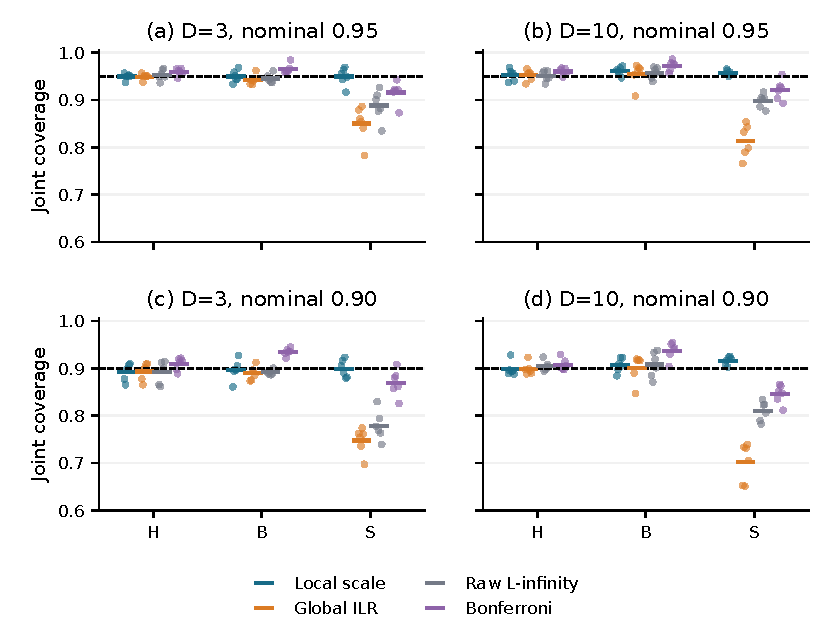
\includegraphics[width=\textwidth]{figures/coverage_by_condition.pdf}
\caption{Joint coverage by condition, dimension, and nominal level. Small dots show individual seeds; horizontal colored marks show means; dashed lines show nominal coverage. H: homoscedastic; B: boundary-concentrated heteroscedastic; S: B response mechanism with shifted test covariates. Panels share an axis spanning all observations. Shifted coverage is an empirical stress test, not a validity guarantee.}
\label{fig:coverage}
% @evidence[[paper_data.json#/final_evaluation/evaluation_evidence/episodes]]
\end{figure}

In B3 and B10, local utility rises to 0.89045 and 0.90820, compared with global utilities 0.84703 and 0.84162. The contrast is not merely a pooled score effect: fixed-group error decreases from 0.07770 to 0.01816 in B3 and from 0.07181 to 0.01723 in B10. Reference mass also decreases, from 0.47580 to 0.39349 and from 0.49497 to 0.32211. Local mean coverage at nominal 0.90 is 0.89689 in B3 and 0.90706 in B10. These joint observations support improved allocation under the evaluated heteroscedastic mechanism, while the remaining discrepancies preclude claiming exact conditional calibration.
% @evidence[[analysis_summary.json#/cases/B3]]
% @evidence[[analysis_summary.json#/cases/B10]]
% @evidence[[paper_data.json#/final_evaluation/evaluation_evidence/episodes]]

Raw-coordinate methods are useful alternatives rather than uniformly weak baselines. Bonferroni is conservative in these heteroscedastic conditions: at nominal 0.90 its mean coverage is 0.93465 in B3 and 0.93717 in B10. Its group errors are lower than global ILR's but higher than the local procedure's. Raw $L_\infty$ also improves some global-ILR summaries without matching the local procedure's aggregate tradeoff. The comparison concerns complete region constructions. It cannot separate coordinate geometry, calibration multiplicity, and learned adaptation into isolated causal contributions.
% @evidence[[analysis_summary.json#/cases/B3]]
% @evidence[[analysis_summary.json#/cases/B10]]

\subsection{Shift Stress Test and the Cost of Coverage Repair}
The shift exposes a substantial gap between global calibration and local scaling in the recorded data. At nominal 0.90, global ILR covers 0.74748 of responses in S3 and 0.70190 in S10; local scaling covers 0.89933 and 0.91610. At nominal 0.95 the corresponding global means are 0.85067 and 0.81405, versus local means 0.94979 and 0.95768. The raw-coordinate baselines mitigate some of this undercoverage but do not reach the same mean coverage in these conditions. This is evidence about the specified covariate shift, not evidence that ordinary split conformal becomes valid under arbitrary shift.
% @evidence[[analysis_summary.json#/cases/S3]]
% @evidence[[analysis_summary.json#/cases/S10]]
% @evidence[[paper_data.json#/final_evaluation/evaluation_evidence/episodes]]

\begin{figure}[t]
\centering
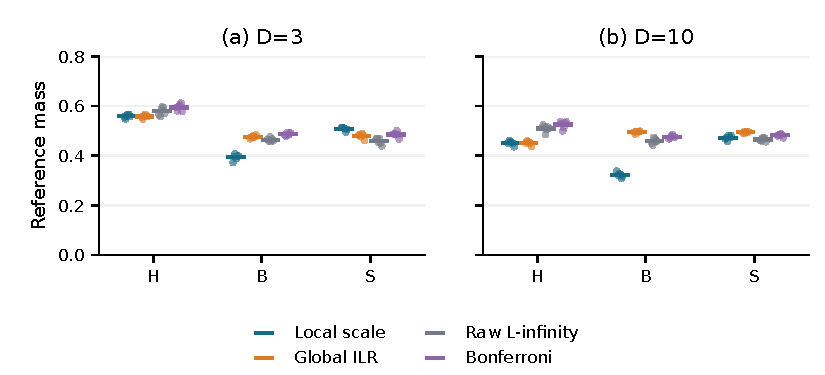
\includegraphics[width=\textwidth]{figures/reference_mass_by_condition.pdf}
\caption{Reference mass, averaged over the two nominal levels within each seed. Dots show seeds and marks show means under the shared mixed reference measure. The S3 local region has greater mass than global ILR; improved coverage must not be summarized as uniformly smaller regions. These values are not intrinsic simplex volumes.}
\label{fig:mass}
% @evidence[[paper_data.json#/final_evaluation/evaluation_evidence/episodes]]
\end{figure}

Figure~\ref{fig:mass} makes the efficiency qualification explicit. S3 local mass is 0.50795, exceeding global ILR's 0.47945. A global region that misses many shifted responses can look artificially economical. Local scaling pays additional mass while restoring empirical coverage in that condition. S10 instead has local mass 0.47159 versus global mass 0.49482. The two outcomes rule out a uniform region-size claim even within this limited evaluation. They also illustrate why mass and coverage should be inspected together rather than collapsing the interpretation into one scalar.
% @evidence[[analysis_summary.json#/cases/S3]]
% @evidence[[analysis_summary.json#/cases/S10]]

\subsection{Alignment Controls and Attribution Limits}
The constant-covariate control agrees with global ILR, with aggregate utility 0.82960. Permuting training residual targets gives utility 0.82985, compared with 0.87723 for aligned local scaling; the paired interval for the aligned-minus-permuted utility difference is [0.04313, 0.05109]. This comparison supports the relevance of covariate--residual alignment to the complete procedure under this design. Permutation also changes model selection and estimation, so it does not isolate a particular functional component. All declared control checks pass in the final record, which is a diagnostic result rather than a separate scientific guarantee.
% @evidence[[paper_data.json#/final_evaluation/metrics]]
% @evidence[[paper_data.json#/final_evaluation/evaluation_evidence/episodes/0/solution/paired_seed_intervals/permuted]]

The quantile-stump family, ridge fallback, offsets, and selection are evaluated together. Missing selection diagnostics and the matched final ridge-only comparison prevent attributing gains to stumps. Similarity to global calibration in H does not identify the selected component.

\section{Discussion and Limitations}
The results favor local scaling when covariates carry information about residual magnitude, but this conclusion is bounded in several ways. The synthetic response law is deliberately well aligned with scalar adaptation in ILR coordinates. Its center is linear and its conditional noise is isotropic. A scalar cannot learn direction-specific residual geometry, multimodality, or systematic center misspecification. The evaluation does not establish what would happen if those features dominated. Likewise, because boundary concentration and heteroscedasticity change together between H and B, we cannot attribute the benefit to the boundary itself.

The validity distinction is structural. Under exchangeability, training-only selection can change efficiency without invalidating the calibration rank argument. Fixed-group diagnostics assess practical heterogeneity but do not strengthen that theorem. Under the S shift, a plausible normalization mechanism can explain favorable empirical behavior without proving exchangeability of the learned normalized scores. Density-ratio weighting or other shift-aware calibration would require a different evaluated method. We make no claim that local scaling replaces those techniques.

The size proxy is also a scientific choice. Our shared mixture balances a training-residual-based local reference and a uniform-simplex reference, so it makes matched comparisons reproducible. It does not define a representation-independent notion of optimal set size. Different reference distributions or reliability weights might change rankings. No weight-sensitivity experiment is available. The chosen utility penalizes overcoverage and undercoverage equally, which may not match an application where missing a response is much more costly than a conservative set.

The empirical scope is narrow: continuous, strictly positive synthetic compositions at two dimensions and two nominal levels. Exact zeros, sparse count responses, real topic proportions, and estimated class-probability vectors are not evaluated. A prediction region for the observed continuous response is not automatically a confidence region for a latent composition. Nor do the results compare label-set classification methods. Six seeds quantify repeatability only coarsely; the bootstrap cannot recover unobserved distributional diversity or correct selection biases outside the frozen final assessment.
% @evidence[[paper_data.json#/final_evaluation/evaluation_evidence/episodes]]

Readable source evidence supports the implementation description, but its documentary linkage is not an independently recomputed frozen source-tree identity proof. Missing component diagnostics and the matched final learned-ridge comparator limit mechanism-level attribution; supplementary material records source locations and incomplete extensions.

\section{Conclusion}
Training-only local residual scaling offers a useful but conditional improvement for joint conformal prediction of continuous compositions. In the evaluated logistic-normal conditions, the complete scale-selection procedure improves the aggregate coverage--reference-mass tradeoff over global ILR and raw-coordinate comparators. The clearest benefits occur under boundary-concentrated heteroscedasticity, whereas homoscedastic controls provide no consistent advantage. The shifted conditions show favorable empirical coverage, but one condition requires more reference mass and neither establishes distribution-shift validity.

The methodological lesson is to distinguish the marginal guarantee supplied by calibration, the allocation of region size supplied by the score, and empirical usefulness. Utility cannot replace that separation. Anisotropic responses, real compositions, alternative reference measures, and controlled component comparisons remain open tests. The supported claim is condition-dependent usefulness of the complete scale procedure, not quantile-stump superiority or universal efficiency.

\clearpage
\bibliographystyle{paper}
\bibliography{references}
\clearpage
\appendix
\section{Supplementary Information}
\subsection{Synthetic Generator and Frozen Partitions}
The original synthetic generator is task-owned and requires no downloaded dataset, account, or external data license. For each dimension the coefficient matrix is fixed, while independent seed lineages generate examples. The evaluator's contrast basis has column $j$, for zero-based $j$, equal to $1/\sqrt{(j+1)(j+2)}$ in the first $j+1$ entries, $-(j+1)/\sqrt{(j+1)(j+2)}$ in entry $j+1$, and zero elsewhere. This gives an orthonormal basis of the zero-sum subspace and hence an invertible ILR representation on strictly positive compositions.

The four partition sizes, in center/scale/calibration/test order, are $(1024,1024,512,2048)$. The S shift applies only to the test partition. The stored raw-generation manifest identifies the example lineages and disjointness checks; these identifiers establish provenance, not extra measurements. The split-conformal theorem uses independence of fitting from calibration and exchangeability of calibration with a new response; it does not require that every partition have equal size.
% @evidence[[source_evidence/final_manifest.json#/files/0/sizes]]
% @evidence[[source_evidence/evaluate_final.py#L566-L624]]

\subsection{Scale Family and Selection Details}
Readable source evidence is included at \texttt{source\_evidence/scale\_learner.py}. Lines 64--74 define feature and pinball-loss utilities; lines 90--134 fit additive quantile stumps; lines 143--155 define the standardized quadratic ridge model; lines 158--178 define candidate blends and fitting-only alignment; and lines 181--213 implement fold-local model selection and full-data refitting. The entry specification identifies a Python script at \texttt{program.py}; the supplied source copy preserves the evaluated-interface implementation for inspection.

The ridge log target uses a residual floor of $10^{-8}$, while the tail target uses $10^{-12}$. Standard deviations for covariate standardization are floored at $10^{-8}$. The ridge intercept penalty is $10^{-8}$ rather than exactly zero. Prediction clips ridge log scales before blending and clips the final exponent argument to $[-30,30]$ before applying a positive floor. The evaluator then applies its common scale clipping. These are numerical details, not evidence that saturation never occurs; no saturation diagnostic is recorded.
% @evidence[[source_evidence/scale_learner.py#L143-L225]]

The selection rule estimates standard error from fold losses using their sample standard deviation divided by the square root of the number of folds. Fold losses are dependent through overlapping fitting partitions, so the rule is a conservative model-selection heuristic, not a calibrated hypothesis test. All offsets are fitted inside their respective fitting partitions. Neither offsets nor fold losses use conformal-calibration responses. The final fit reconstructs the candidate family regardless of which index is selected.

\subsection{Extended Metrics and Between-Seed Variation}
Table~\ref{tab:case} expands the utility comparison. Standard deviations describe variability across independent seed episodes, not uncertainty in individual membership decisions. The main figures show the corresponding coverage and mass observations without manufacturing condition-specific bootstrap intervals. Table~\ref{tab:group} reports the fixed-group and mass summaries that make the condition-dependent conclusion interpretable.

\begin{table}[h]
\centering
\caption{Condition-specific mean utility $\pm$ sample standard deviation over seeds. Comparisons are matched within each seed; these marginal standard deviations are not paired difference intervals.}
\label{tab:case}
\begin{tabular}{lrrrr}
\toprule
Condition & Local & Global ILR & Raw $L_\infty$ & Bonferroni\\
\midrule
H3 & $0.8532\pm0.0046$ & $0.8533\pm0.0046$ & $0.8455\pm0.0035$ & $0.8422\pm0.0063$\\
H10 & $0.8789\pm0.0047$ & $0.8803\pm0.0045$ & $0.8655\pm0.0049$ & $0.8601\pm0.0075$\\
B3 & $0.8904\pm0.0049$ & $0.8470\pm0.0038$ & $0.8564\pm0.0035$ & $0.8519\pm0.0033$\\
B10 & $0.9082\pm0.0058$ & $0.8416\pm0.0128$ & $0.8593\pm0.0022$ & $0.8530\pm0.0053$\\
S3 & $0.8604\pm0.0047$ & $0.7924\pm0.0154$ & $0.8204\pm0.0139$ & $0.8445\pm0.0110$\\
S10 & $0.8722\pm0.0044$ & $0.7631\pm0.0210$ & $0.8327\pm0.0075$ & $0.8415\pm0.0090$\\
\bottomrule
\end{tabular}
% @evidence[[analysis_summary.json#/cases]]
% @evidence[[paper_data.json#/final_evaluation/evaluation_evidence/episodes]]
\end{table}

\begin{table}[h]
\centering
\caption{Mean fixed-group absolute error and reference mass for local and global ILR regions, averaging both nominal levels within each seed.}
\label{tab:group}
\begin{tabular}{lrrrr}
\toprule
Condition & $E_g$ local & $E_g$ global & $M$ local & $M$ global\\
\midrule
H3 & 0.01035 & 0.01087 & 0.55883 & 0.55803\\
H10 & 0.01137 & 0.00929 & 0.45106 & 0.45105\\
B3 & 0.01816 & 0.07770 & 0.39349 & 0.47580\\
B10 & 0.01723 & 0.07181 & 0.32211 & 0.49497\\
S3 & 0.01906 & 0.10816 & 0.50795 & 0.47945\\
S10 & 0.01446 & 0.13488 & 0.47159 & 0.49482\\
\bottomrule
\end{tabular}
% @evidence[[analysis_summary.json#/cases]]
\end{table}

The stored paired utility interval against the uncalibrated comparator is [0.04434, 0.04862]. This comparator changes both the sample used to choose a radius and the quantile convention. It therefore does not isolate the numerical finite-sample correction. The comparator's role is a diagnostic for replacing held-out calibration with a training-residual threshold, not a clean ablation of the rank correction alone.
% @evidence[[paper_data.json#/final_evaluation/evaluation_evidence/episodes/0/solution/paired_seed_intervals/uncalibrated]]

\subsection{Controls and Degenerate Regions}
The constant control zeroes covariates during fitting and prediction, making its output independent of covariate location. Its checked equivalence to global ILR validates cancellation of a constant scale in the implemented calibration procedure. The permutation control cyclically shifts residual-target indices and checks that the alignment actually changes; it does not demand a predetermined sign for the resulting utility difference. This is why an individual permuted result is not, by itself, a failed control.

The full-simplex control has coverage and reference mass equal to one throughout the final records. The singleton-center control has observed coverage and reference mass equal to zero in those records. Those are measured membership outcomes in this continuous-response evaluation, not assumed properties to be substituted for measurements. Geometry checks also verify corrected-quantile behavior, including an infinite threshold when the required rank exceeds calibration size. Reset/replay checks test reproducibility of the scale interface, not distribution-free validity.
% @evidence[[paper_data.json#/final_evaluation/evaluation_evidence/episodes]]
% @evidence[[source_evidence/evaluate_final.py#L588-L601]]

\subsection{Conditional Rank Argument and Invariance}
Fix the two fitting samples and let $s_c(x)$ denote the clipped positive scale. The calibration scores and a new score are evaluations of the same deterministic function of exchangeable pairs. If ties are broken randomly for the argument, the new rank is uniform on the available ranks; using a non-strict set threshold can only increase inclusion. The corrected rank in Equation~\ref{eq:calibration} therefore yields the usual lower marginal coverage bound. When the rank exceeds calibration size, the infinite threshold includes every finite-score response, retaining the bound. Nothing in this reasoning requires pinball fitting to recover a true conditional quantile.

For any positive constant $a$, replacing a scale $s$ by $as$ divides every calibration score and its empirical threshold by $a$. The product of threshold and prediction scale is unchanged. This establishes invariance to global scale normalization in the absence of shape-changing clipping. It explains why fitting-set tail alignment need not define the final nominal coverage. It does not imply invariance when clipping differentially saturates covariate-dependent scales. Under shift, the normalized scores may cease to be exchangeable even if their observed mean coverage is close to nominal. A residual-factorization hypothesis would need additional support to justify stronger statements.

\subsection{Reproducibility, Source Linkage, and Evaluation Scope}
The recorded evaluation environment is Linux x86\_64, CPython 3.12, and NumPy 2.1.3, using CPU execution and single-threaded BLAS. These are recorded evaluator settings, not a claim that the present manuscript-building environment is identical. The anonymous reproduction instructions in \texttt{REPRODUCIBILITY.md} identify dependencies, seeds, commands, source locations, and figure/table generation. A portable copy of the evaluator, selected learner, and frozen raw resources is supplied under \texttt{reproduction/}; its scientific invocation was not rerun during writing. All plotted numerical data come from the frozen final records in \texttt{paper\_data.json}.
% @evidence[[source_evidence/final_manifest.json#/environment]]
% @evidence[[paper_data.json#/final_evaluation/evaluation_evidence/episodes]]

The included source copies support the implementation description directly. For the evaluator, \texttt{source\_evidence/evaluate\_final.py}, lines 604--624 define the generator, lines 670--705 define intervals and utility, lines 716--774 define center fitting and shared probes, and lines 950--974 define aggregate resampling. The frozen evaluation stores source-tree and evaluator identifiers. We have not independently reconstructed an exact source-tree identity match between every local copy and that frozen tree; hashes alone are not used to justify implementation claims. Candidate-generated component diagnostics remain unverified, and selected-component labels are unavailable.

Two development directions do not provide extra measured evidence for the thesis: a count-noise/latent-target extension was not expressible through the scale-only interface and was not implemented; an interaction-tree extension has an unsuccessful evaluation with no measured score and no identified failure cause. Neither is a measured loss or a successful ablation. We do not infer whether the latter failed statistically, operationally, or because of a validity restriction. Development scores are not compared numerically with final scores, and the absence of a matched final ridge-scale baseline remains a limitation.
% @evidence[[source_evidence/latent_extension_limitations.md]]
% @evidence[[source_evidence/interaction_failure.json]]

The final qualification sources record completion and a qualified outcome, with the declared checks satisfied. No failed final qualification is present in the supplied registry. This status does not certify conditional validity, shift validity, or an explanation of component effects. Missing gate diagnostics are left unknown. The stored elapsed durations include evaluator work and are not reported as isolated learner runtime. New scientific experiments, model refits, and added performance measurements were not run during manuscript preparation.
% @evidence[[paper_data.json#/grounding_sources/final.qualification.status]]
% @evidence[[paper_data.json#/grounding_sources/final.qualification.outcome]]
% @evidence[[paper_data.json#/grounding_sources/final.qualification.correct]]

\subsection*{LLM Usage}
LLM assistance was used for research proposal formulation, implementation drafting, reference-query planning, and manuscript framing in the supplied workflow. During preparation of this manuscript, an LLM inspected the structured evaluation records and readable source files, generated plotting and table scripts, consulted directly identified reference metadata and abstracts, drafted text and claim mappings, and repaired validation issues. Numerical results were taken from existing frozen evaluation artifacts rather than generated by the language model. LLM assistance is not an independent scientific validation or an author identity claim. No undocumented model version or unrecorded human verification is asserted. Literature access was restricted to directly identified foundational sources and their metadata or abstracts; no prohibited-literature encounter was documented during this manuscript step.

\end{document}
